\documentclass{article}
\thispagestyle{empty}
\usepackage{graphicx}
\usepackage{tikz}
\usetikzlibrary{decorations.pathreplacing}
\begin{document}
\begin{figure}
  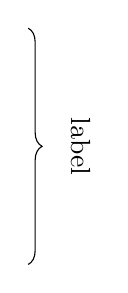
\begin{tikzpicture}
%    \draw[decoration={brace, amplitude=5pt}, decorate] (0, 0) -- node[sloped, above=12pt] {label} (0, 3);
    \draw[decoration={brace, amplitude=5pt}, decorate] (2, 3) -- node[sloped, above=12pt] {label} (2, 0);

  \end{tikzpicture}
\end{figure}
\end{document}
